\frame {
    \frametitle{\LARGE Общие сведения: Цепи Маркова (1/3)}
    \vskip2em
    \begin{columns}
        \begin{column}{0.4\textwidth}
            \begin{itemize}
                \item[---] с дискретным временем;
                \item[---] с непрерывным временем;
                \item[---] скрытые Марковские модели;
            \end{itemize}
        \end{column}
        \begin{column}{0.5\textwidth}
            \begin{center}
$$
  P =
  \begin{bmatrix}
    1 & 0 & 0     \\
    1/2 & 0 & 1/2 \\
    2/3 & 0 & 1/3
  \end{bmatrix}
$$

            \vskip.5em
            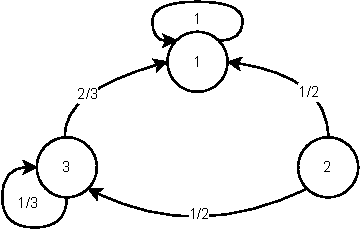
\includegraphics[scale=0.5]{inc/img/markov-chain.pdf}
%            \vskip.5em
%            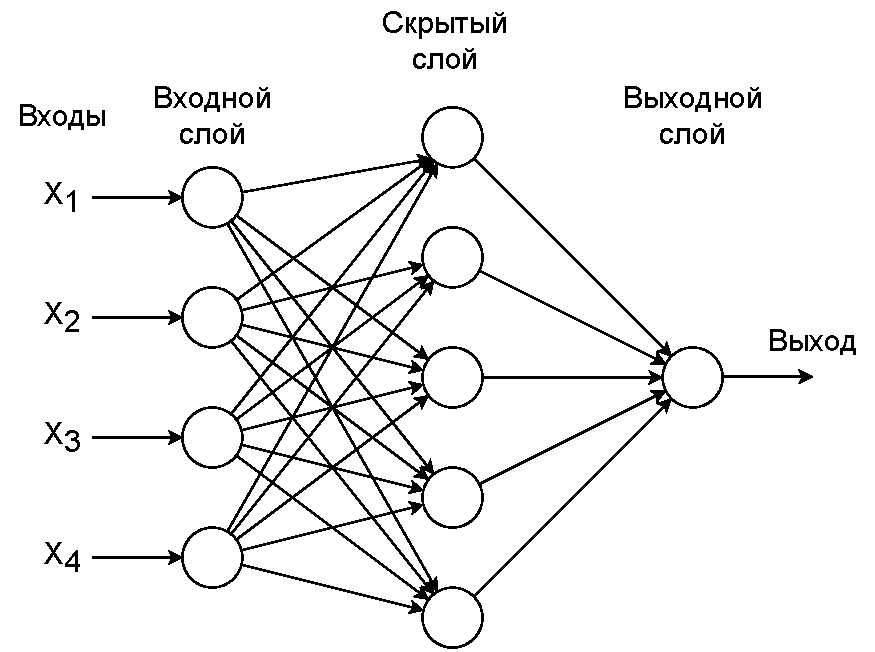
\includegraphics[scale=0.3]{inc/img/network.pdf}
            \end{center}
        \end{column}
    \end{columns}
}
